\section{Methodology}


\subsection{Design}

The design of the project involves the following aspects. 

\subsubsection{Architecture Overview}

Our proposed pipeline consists of four major modules, including the following:

\paragraph{Document Preprocessing}
We preprocess documents into the expected format before embedding and storage into the knowledge base.
This step performs text splitting into overlapping chunks, and inline image extraction and context-aware captioning.

\paragraph{Dual-Representation Database Storage}
We maintain two separate indexes, with one for text chunks, and the other as a multi-vector database for image features and captions.
The text index may be a vector database if dense retrieval is selected in the configurations,
or a knowledge graph of entities and relationships when graph retrieval mode is chosen.

\paragraph{Multimodal Retrieval}
Retrieval takes on three modes (text-to-text, text-to-image, and image-to-image), depending on the modalities of the input query.
Dense retrieval uses cosine similarity between embeddings, while graph retrieval extracts the most relevant communities in the knowledge graph.

\paragraph{Grounding Generation}
Retrieved texts and images form a final prompt with the raw query.
The final prompt is then passed to a MLLM to produce a final answer conditioned on retrieved evidence,
ensuring accuracy by grounding on external knowledge as context.

\subsubsection{Design Principles}
Our project objectives guide all pipeline decisions.

We preserve fine-grained details in each modality (text and visual), and choose methods that keep each modality processed 
in their respective representation spaces.
By using dual representations instead of flattening representations into a single embedding space,
we allow for robust text features and fine-grained visual details to both be leveraged in retrieval and grounding generation.

Our pipeline provides a training-free multimodal RAG solution, leveraging existing pretrained foundation models,
including MiniLM text embedding models \cite{10.5555/3495724.3496209}, DINOv2, an image feature extraction model \cite{oquab2024dinov2learningrobustvisual},
and Talk2DINO, a mapping model that translates text embeddings into the image feature space \cite{Barsellotti_2025_ICCV}.
This ensures reproducibility, simplicity in application, and controllable computational cost.

The configurable storage option between using a vector database and knowledge graph storage enables pipeline choice depending on actual usage needs.
Vector database and dense retrieval provide fast and scalable storage and retrieval,
while knowledge graph storage may offer better handling for long-context relations; though our experiments did not confirm this advantage.

Generation grounding on both textual and visual modalities is supported, ensuring accuracy with the most retrieved evidence.

\subsubsection{Design Tradeoffs}

We utilize DINOv2 \cite{oquab2024dinov2learningrobustvisual} as our visual feature extractor, 
for its superior fine-grained visual detail preservation from self-supervised learning.
Although it does not provide a natural language interface, we utilize an additional layer Talk2DINO \cite{Barsellotti_2025_ICCV}
to map text tokens into the same representation space, incurring slightly more computation.

As for cross-modal alignment, CLIP \cite{radford2021learningtransferablevisualmodels} inherently provides an alignment mapping
between open-vocabulary natural language and visual content.
However, surveys on existing multimodal RAG methods which mainly make use of CLIP for multimodal alignment reveal that
CLIP-based vision encoding does not capture fine-grained visual details in images, or demonstrates a bias towards text 
instead of multimodal elements \cite{abootorabi-etal-2025-ask,lin2025mmembeduniversalmultimodalretrieval}.
We hence use Talk2DINO \cite{Barsellotti_2025_ICCV} to align text queries with DINOv2's fine-grained visual features.

During retrieval, we generate a zero-shot answer to the input query to assist in retrieval.
Since user queries may be brief, the hypothetical document often contains textual patterns commonly found in the expected domain and answer,
hence achieving higher recall in retrieval.
This is known as the Hypothetical Document Embeddings (HyDE) technique \cite{gao-etal-2023-precise} (more details in Section~\ref{sec:retrieval} \nameref{sec:retrieval}).
Although hallucinated details may be introduced and propagated to the final answer,
we adopt this method as the final answer remains grounded on real retrieved documents.

\subsubsection{Design Validation}

We validate design decisions using unit tests and integration tests (detailed tests and results in Section~\ref{sec:testing} \nameref{sec:testing}).
Unit tests examine the capabilities of independent components of our pipeline using mock generated data,
to verify that our pipeline components operate on input documents as expected.
Integration tests examine the entire pipeline end-to-end, to examine actual results on small datasets for easy verification that
the pipeline gives good performance.

Benchmark comparisons (in Section~\ref{sec:evaluation} \nameref{sec:evaluation}) compare our full pipeline against methods developed in previous work.
We examine our pipeline's performance with the benchmarks Visual-RAG \cite{wu2025visualragbenchmarkingtexttoimageretrieval}
and MMDocRAG \cite{dong2025benchmarking}.


\subsection{Implementation}

The implementation of this project involves: 

\subsubsection{Dataset Collection}

This project aims to explore a generic RAG pipeline that supports multimedia to be used as context in multimodal LLMs.
As such, we collect and utilize datasets provided by publicly available benchmarks, to ensure wide domain and topic coverage.

\paragraph{Visual-RAG}
Visual-RAG \cite{wu2025visualragbenchmarkingtexttoimageretrieval} is a benchmark that explicitly requires text-to-image retrieval 
to answer queries and visually grounded generation with retrieved visual evidence.
Benchmark dataset is based on the iNaturalist 2021 \cite{Van_Horn_2021_CVPR} dataset containing 2.7M images from 10,000 different species.
We utilize this benchmark to evaluate our pipeline's retrieval accuracy based on very fine-grained visual details.

\paragraph{MMDocRAG}
MMDocRAG \cite{dong2025benchmarking} features over 4,000 expert-annotated question-answer pairs that rely on multi-page or multi-document cross-modal evidence.
As visual evidence is a core evaluation metric in this benchmark, we evaluate our pipeline on this benchmark to compare with other models or methods,
and to identify limits and guide future improvements.

We use these benchmarks to evaluate both retrieval and end-to-end answer generation using the final answer.
Since our prompts (listed in Appendix~\ref{appendix:prompts} \nameref{appendix:prompts}) instruct the MLLM to answer only based on retrieved context,
the final answer also reflects retrieval accuracy in a unified evaluation score.

\subsubsection{Document Preprocessing}

Input documents involve text and inline images.
Our pipeline separates text and images in input documents for preprocessing, and fuses them partially for easy reference between relevant items.

As industry-grade documents can contain long content of up to hundreds of pages,
we split document text into processable sizes. 
Input documents are first split into text chunks of fixed length with pre-defined fixed overlap \cite{bansal2023optimizingragchunking},
by recursive splitting of text to avoid cutting text mid-word into different chunks.
The length and overlap between chunks are configurable constants. 

As for images, we extract them from the document alongside text surrounding the inline image.
We perform captioning for inline images using the extracted context from source documents to support captioning,
such that document context is preserved when processing images in later steps.
From testing different approaches (see Section~\ref{sec:captioningtests} \nameref{sec:captioningtests} for details, results, and analysis),
we find that using MLLMs for captioning images provides the best tradeoff between computation cost and accuracy.

Chunks of text, their metadata, and images with their metadata are passed on to the next step in the pipeline for embedding.

\subsubsection{Embedding}

Chunks of text obtained from the preprocessing step are then embedded using a text encoder that maps short sentences or paragraphs 
into a high-dimensional dense vector space.
The MiniLM models \cite{10.5555/3495724.3496209}
\footnote{The original paper gives details on training and the performance of the base model \verb|microsoft/MiniLM-L12-H384-uncased|.
In this project, we use a more powerful model, \verb|sentence-transformers/all-MiniLM-L6-v2|, 
which is a fine-tuned version of the base model with a contrastive learning objective on a large dataset of sentences pairs.}
distilled from BERT \cite{devlin-etal-2019-bert} provide ideal performance in extracting semantic features from short texts into dense vectors.
We use a MiniLM model to embed chunks of text and store the obtained dense vectors at preprocessing time, 
and encode queries into dense vectors in the same space to search in the knowledge base for similar text vectors.

Embedding multimedia data cannot be performed with the same method. 
Prior to embedding, each image is extracted for captioning conditioned on source document context surrounding the image using a multimodal LLM. 
Within the source document, the image is replaced with the obtained caption, 
to obtain a fully textual of the document for embedding with the above methods. 

To obtain embeddings of images, we use a generic vision model that extracts visual features into dense feature vectors.
DINOv2 \cite{oquab2024dinov2learningrobustvisual} is a foundational vision model trained by self-supervision and gives feature vectors of images.
We utilize DINOv2 in embedding images. 
Image embeddings are then placed in a vector database storage separate from the processed text embeddings, 
and similar or relevant items are linked to each other via metadata. 

\begin{figure}
    \centering
    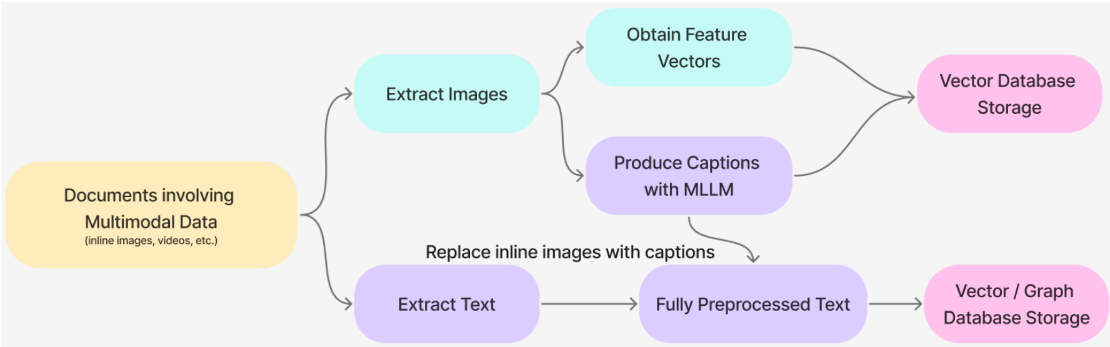
\includegraphics[width=\textwidth]{images/2-method/embedding-flow.png}
    \caption{Flow of embedding input data and storage in knowledge base}
\end{figure}

\subsubsection{Storage}

Chunks of processed data are embedded into text embedding vectors and stored in an external knowledge base.
This is implemented using a vector database that provides storage and quick query functions. 

Image feature vectors are stored in a separate vector database; with the difference being that a multi-vector database is used. 
Image vectors and caption embeddings are connected to each other during storage, to allow text queries to also be used during the retrieval process. 

An alternate storage framework using knowledge graphs has also been implemented, following \cite{edge2025localglobalgraphrag}. 
Using graph storage is an option to be chosen in the configurations.
Entities are extracted from source document texts and form nodes in the graph, and relationships between entities form graph edges. 
This is extended to be connected with the image vector database through entity metadata. 
Communities of nodes in the knowledge graph are detected using Louvain's algorithm, 
and community summaries are generated for each community using an LLM. 

\subsubsection{Retrieval}
\label{sec:retrieval}

User queries to an MLLM may involve text only, or both text and reference images or documents. 
Processed documents stored into the knowledge base may contain references or correct answers to the query, 
hence relevant items are retrieved from the database to augment and ground generation to retrieved evidence. 

Prior to retrieval, we offer an option to enhance the user's raw query using the Hypothetical Document Embeddings (HyDE) technique \cite{gao-etal-2023-precise}.
A zero-shot prompt is first generated as a hypothetical document without any context and purely based on the query,
and is then used for retrieval from the external vector database.
While the generated hypothetical document may be highly incorrect and contain numerous hallucinations,
the generated document contains the semantic nuances and patterns of texts on the same topic or domain.
This text is then embedded using the same text encoder used in processing external documents,
and the obtained embeddings are then used for text-to-text retrieval.
Since our tests show no significant advantage in using HyDE (see Section~\ref{sec:ablationtests} \nameref{sec:ablationtests} for results and analysis),
we leave this as a configurable option.

User queries may involve both text and images.
While image-to-image can simply be done through passing query images through the same DINOv2 model to obtain a feature vector to perform dense retrieval,
cross-modal retrieval by using text to retrieve images requires further steps.
CLIP \cite{radford2021learningtransferablevisualmodels} unifies feature vector representations of text and images,
yet it does not provide accurate visual features existing in models.
Talk2DINO \cite{Barsellotti_2025_ICCV} provides a projection layer from the CLIP embedding space to the DINOv2 embedding space,
bridging the gap between text features and visual features vector spaces.
Talk2DINO was trained by freezing both CLIP and DINOv2 backbones and achieves state-of-the-art results, 
hence we utilize this approach in performing cross-modal operations.

Queries for text-to-image cross-modal retrieval may be long to contain more expected content in images.
The original CLIP model, used in Talk2DINO to encode text, suffers from a context size limit of 77 tokens, 
which is largely limited in this detailed retrieval use case if detailed visual elements are concerned.
We hence utilize Long-CLIP \cite{10.1007/978-3-031-72983-6_18} as the text encoder in the cross-modal retrieval step,
to support longer queries that involve more detailed descriptions of expected visual features.

Following from the embedding and storage methods used, cosine similarity between vector embeddings is the primary retrieval criteria. 
Retrieval is performed through the following components: 

\begin{itemize}
    \item \textbf{Text-to-text search}: 
        Query text to retrieve similar text chunks from the textual vector database using text embedding cosine similarity.
    \item \textbf{Image-to-image search}: 
        Images in the query, if any, are passed through the image feature extraction model to obtain a feature vector.
        This feature vector is then used to search for similar images in the image multi-vector database, using cosine similarity between image feature vectors.
    \item \textbf{Text-to-image search}: 
        Query text is embedded into the DINOv2 embedding space using Talk2DINO \cite{Barsellotti_2025_ICCV}, 
        a model that aligns text embeddings into the visual feature vector space of DINOv2 \cite{oquab2024dinov2learningrobustvisual}. 
        Similarly, images are retrieved using cosine similarity between the aligned text embeddings and image feature vectors.  
\end{itemize}

When the graph-based storage method option is chosen, text-to-text search is implemented differently.
The user query and community summaries are embedded with the same MiniLM text embedding model.
We compare the relevance of a community by the cosine similarity between embeddings of the user query and the community summary.
Since we consider the top $k$ most relevant items, we retrieve the $k$ communities with the highest cosine similarity scores with the user query.
We then aggregate the summaries of these communities as the retrieval result and provide an answer to the query.

\begin{figure}[H]
    \centering
    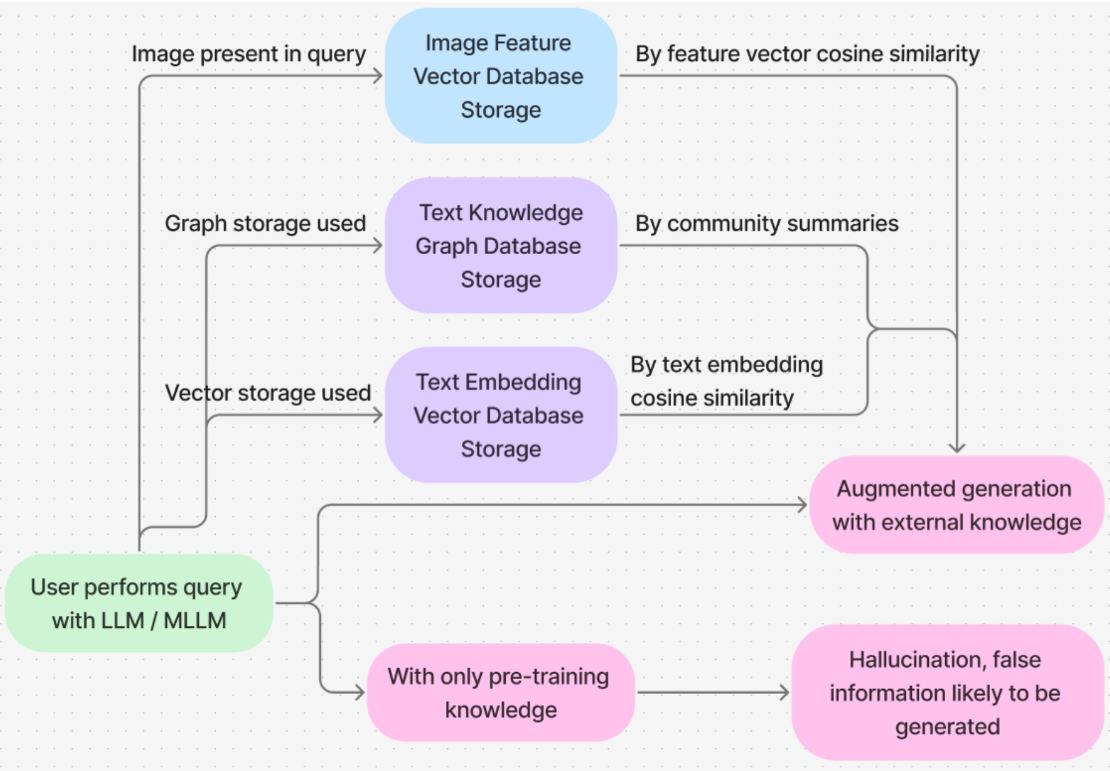
\includegraphics[width=0.8\textwidth]{images/2-method/high-level-overview.png}
    \caption{A high level overview of the entire project and implementation}
\end{figure}

\subsubsection{Formal Task Definition}

Given a set of $n$ documents $\mathcal{D} = \{ d^{(i)} \}_{i=1}^n$, 
where each document $d^{(i)}$ is composed of text $t^{(i)}$ and a set of $p$ images $\mathcal{I}^{(i)} = \{m_j^{(i)}\}_{j=1}^p$,
the following steps are carried out.

\paragraph{Image Captioning}
Each image extracted from the document is first captioned using an MLLM using text surrounding the image $t^{(i)}_{m_j^{(i)}}$ as context.
\begin{equation}
    \mathcal{P}^{(i)} = \{p_j^{(i)} \mid p_j^{(i)} = \text{MLLM}(x \mid \mid t^{(i)}_{m_j^{(i)}} \mid \mid m_j^{(i)})\}
\end{equation}
where $x$ is the prompt instructing the MLLM to provide captions, and $\mid \mid$ indicating concatenation into the full prompt.
The captions $\mathcal{P}^{(i)}$ are then inserted back into the text in the corresponding image position before further textual processing.

\paragraph{Chunking}
The text in the document is first split into chunks of fixed size $L$ with a fixed overlap of $O$ characters between consecutive chunks.
Let $t_\text{combined}^{(i)} = t^{(i)} \cup \mathcal{P}^{(i)}$ be the full text with inserted image captions.
The chunking process creates overlapping chunks indexed from $j = 0$ to $m$, where:
\begin{equation}
    c_j^{(i)} = t_\text{combined}^{(i)}[s_j : e_j]
\end{equation}
with start and end positions:
\begin{equation}
    \begin{split}
        s_j &= j \cdot (L - O) \\
        e_j &= s_j + L
    \end{split}
\end{equation}
where $L$ is the chunk size and $O$ is the overlap length.
Adjacent chunks $c_j^{(i)}$ and $c_{j+1}^{(i)}$ share $O$ characters of overlap to preserve context.
The total number of chunks is $m = \lceil \frac{|t_\text{combined}^{(i)}| - L}{L - O} \rceil + 1$.

\paragraph{Embedding and Storage}
Each chunk is embedded into a vector $\mathbf{v}_j^{(i)}$ using a neural text embedding model $\mathcal{N}_{\text{text}}$.
\begin{equation}
    \mathbf{v}_j^{(i)} = \mathcal{N}_{\text{text}}(c_j^{(i)})
\end{equation}
These vectors are stored into an external vector database $\mathcal{S}$.

Alternatively in the graph-based storage option, first use an LLM to extract entities and relationships between entities from the source text.
Entities form a set of nodes $N$ in the graph, and relationships form edges $E$ in the graph.
The graph is formed as
\begin{equation}
    \mathcal{G} = (N, E)
\end{equation}
Using Louvain's Algorithm, we locate communities $C = \{C_1, C_2, ...\}$ in the graph and provide a community summary for each community using an LLM.
\begin{equation}
    C_{\text{summaries}} = \{\mathrm{LLM}(C_j)\}
\end{equation}

Images are embedded using an image feature extraction model, DINOv2, to obtain image embeddings.
\begin{equation}
    \mathbf{g}_j^{(i)} = \mathrm{DINOv2}(m_j^{(i)})
\end{equation}
Image embeddings and their caption embeddings will then be stored into a multi-vector database $\mathcal{S}_{\text{images}}$ as tuples:
\begin{equation}
    \left(\mathbf{g}_j^{(i)}, p_j^{(i)}\right)
\end{equation}

\paragraph{Retrieval}
Retrieval is performed using a user query $\mathcal{Q} = \left(q_{\text{text}}, \mathcal{Q}_{\text{images}}\right)$, 
which is a tuple of query text and a set of query images.
We consider top $k$ items retrieved, and $\mathrm{sim}(\cdot, \cdot)$ as the similarity metric.

\begin{itemize}
    \item Using the query text, first retrieve $k$ text chunks that have the highest embedding similarity with the query.
        \begin{equation}
            \mathcal{C}^R = \{\mathbf{v}_j^{(i)} \in \mathcal{S} \mid j \in \text{top-}k \text{ indices} (\mathrm{sim}(\mathbf{v}_j^{(i)}, \mathcal{N}_{\text{text}}(q_{\text{text}})))\}
        \end{equation}
    \item If there are images in the query, i.e. $\mathcal{Q}_{\text{images}} \neq \emptyset$, obtain a feature representation for each image $q_{\text{images}}$ and retrieve similar images.
        \begin{equation}
            \mathcal{I}^R = \bigcup_{q_{\text{images}} \in \mathcal{Q}_{\text{images}}} \{\mathbf{g}_j^{(i)} \in \mathcal{S}_{\text{images}} \mid j \in \text{top-}k \text{ indices} (\mathrm{sim}(\mathbf{g}_j^{(i)}, \mathrm{DINOv2}(q_{\text{images}})))\}
        \end{equation}
    \item Finally, the cross-modal retrieval step by embedding the query text in DINOv2 feature vector space and retrieve similar images.
        \begin{equation}
            \mathcal{I}^R = \mathcal{I}^R \cup \{\mathbf{g}_j^{(i)} \in \mathcal{S}_{\text{images}} \mid j \in \text{top-}k \text{ indices} (\mathrm{sim}(\mathbf{g}_j^{(i)}, \mathrm{Talk2DINO}(q_{\text{text}})))\}
        \end{equation}
\end{itemize}

Under the graph storage option, items are retrieved by scoring community summaries against the query. 
First, we embed the query text and each community summary:
\begin{equation}
    \mathbf{q}_{\text{embed}} = \mathcal{N}_{\text{text}}(q_{\text{text}})
\end{equation}
\begin{equation}
    \mathbf{s}_j = \mathcal{N}_{\text{text}}(C_{\text{summaries}}[j]) \quad \forall C_j \in C
\end{equation}

For each community, we compute a relevance score indicating the usefulness of that community summary in answering the query:
\begin{equation}
    s_j = \mathrm{sim}(\mathbf{q}_{\text{embed}}, \mathbf{s}_j) \quad \forall j
\end{equation}

Communities are ranked by their relevance scores in descending order, and the top $k$ communities are selected for retrieval:
\begin{equation}
    C^R = \{C_j \mid j \in \arg\max_{\text{top } k}(s_1, s_2, \ldots, s_{|C|})\}
\end{equation}
where $\arg\max_{\text{top } k}$ returns the indices of the $k$ largest scores.
The selected community summaries are then aggregated to provide context for answer generation.

\paragraph{Generation}
Output generation is performed with an MLLM by conditioning generation on retrieved text and images.
The final answer $a$ is generated by concatenating retrieved text, query text, retrieved images, and query images.

In dense vector retrieval mode, this is formulated as 
\begin{equation}
    a = \mathrm{MLLM}(\mathcal{C}^R \mid \mid q_{\text{text}} \mid \mid \mathcal{Q}_{\text{images}} \mid \mid  \mathcal{I}^R)
\end{equation}

For graph retrieval mode,
$\mathcal{C}^R_{\text{graph}} = \{(C_{\text{summaries}}[j], E_j^{\text{key}}) \mid j \in \arg\max_{\text{top } k}(s_j)\}$ 
which is the set of top-$k$ community summaries with their associated key entities $E_j^{\text{key}}$.
We aggregrate all community summaries
\begin{equation}
    \mathcal{C}^R_{\text{aggregated}} = C_{\text{summaries}}[1] \mid \mid C_{\text{summaries}}[2] \mid \mid ... \mid \mid C_{\text{summaries}}[k]
\end{equation}
where $\mid \mid$ indicates a concatenation operation.
Generation is formulated as
\begin{equation}
    a = \mathrm{MLLM}(\mathcal{C}^R_{\text{aggregated}} \mid \mid q_{\text{text}} \mid \mid \mathcal{Q}_{\text{images}} \mid \mid \mathcal{I}^R)
\end{equation}

When grounded with retrieved context and evidence from related source documents, generation variance is greatly reduced;
and timely or inaccessible knowledge outside of model knowledge can be utilized.
This avoids incorrect or out-of-context answers from being generated.

A summary of all the notations used is available at Appendix~\ref{appendix:mathnotations} \nameref{appendix:mathnotations}.


\subsection{Testing}
\label{sec:testing}

We perform unit tests on individual components to ensure sanity checks are passed.
We also implement integration tests to verify that components and the end-to-end pipeline interact with external services (e.g. MLLM API calls) as expected.
In integration tests with actual MLLM calls, we use GPT-4o-mini for tests.

\subsubsection{Unit Tests}

Unit tests are written and conducted with \verb|pytest| version 8.3.4.
The list of components tested independently with unit tests is as follows.

\begin{tabularx}{\textwidth}{@{} l >{\raggedright\arraybackslash}X >{\raggedright\arraybackslash}X @{}}
    \toprule
    \textbf{Component} & \textbf{Tests} & \textbf{Example Test Case} \\
    \midrule
    \endhead
    Document Processor & Load document, text chunking, directory processing (6 tests)
        & Process a directory of documents, expect non-zero number of chunks, expect chunks overlap, expect number of chunks and metadata are equal \\
    Vector Database & Add documents, search documents (4 tests)
        & Insert known string and vector, expect same string to be returned when querying with the vector \\
    Image Storage & Store image, retrieve image data URL (3 tests)
        & Create random image bytes and the corresponding image data URL, store image bytes, expect retrieved data URL to be correct \\
    Text Embedding & Test encode single string and list of strings (2 tests)
        & Encode given strings, expect correct dimensionality, expect correct number of embedding vectors \\
    Multimodal Embedding & Conversion between data URL and PIL image, embed image, embed query, consistency (13 tests)
        & Encode given images, expect correct dimensionality \\
    Graph Storage & Entity and relationship extraction, build community (7 tests)
        & Given known corpus, create a graph from entities and relationships extracted, expect graph with non-zero number of nodes and edges \\
    Graph Retriever & Retrieve entity, search global question (7 tests)
        & Given a graph with given entities and relationships, search and retrieve items, expect correct items to be retrieved \\
    Main class & Methods in the main entrypoint class (10 tests)
        & Initialize system, ingest documents, query \\
    End-to-end pipeline & Interaction between components (10 tests)
        & Run through entire pipeline from initialization to query \\
    \bottomrule
\end{tabularx}

We also test edge cases.
Adding empty documents for processing in the vector database or graph storage are tested to be handled correctly without error.
Conversions between image data URLs and PIL images with invalid data URLs are also examined and shown to fail gracefully as expected. 

Among all 62 unit tests, the passing rate is 100\%.

\subsubsection{Image Extraction and Captioning}
\label{sec:captioningtests}

We select 4 documents\footnote{The documents are linked as follows: \\
\url{https://math.libretexts.org/Bookshelves/Calculus/Calculus_(OpenStax)/05\%3A_Integration/5.01\%3A\_Approximating_Areas} \\
\url{https://www.apple.com/hk/en/newsroom/2025/11/apple-intelligence-expands-to-new-languages-including-traditional-chinese/} \\
\url{https://cse.hkust.edu.hk/pg/research/projects/saikit/underwater-slam/} \\
Note: One of the documents was an email from HKUST to university members and is not publicly available.} 
from the Internet to perform integration tests.
These documents contain inline images covering specific mathematics figures, conceptual images in advertisements, informational images with text, 
and images with advanced concepts that require document context to explain. 

Preprocessing by captioning inline images in documents is required in the pipeline. 
We perform integration tests on captioning in-document images with various methods, 
to test the image extraction process, and examine the quality and coherence of captions generated for each image, as well as the time used. 

\paragraph{CLIP}

In this trial, captions were generated following the model implementation of ClipCap \cite{mokady2021clipcapclipprefiximage}. 
As we observed that incorrect context was given in the captions, 
we refined the captions with an LLM conditioning on document context surrounding the image. 

We note that the refined captions are highly influenced by the CLIP-based model caption, 
and hence out-of-context captions were frequently observed. 

\paragraph{Multimodal LLM}

We perform another test by using a MLLM (GPT-4o-mini) to produce captions for images extracted from documents.
The prompt involved instructions on captioning, the image, and context from the source document surrounding the image. 

A significant improvement in accuracy was observed, at the cost of around 40\% longer processing time with larger variability, 
as compared to the previous method. However, we choose this method for integration with the pipeline. 

\paragraph{Test Results and Statistics}

We employed the following scoring rules in assessing the accuracy of captions generated. 

\begin{itemize}
    \item 0: Completely out-of-context. 
    \item 0.25: Partially correct, but brings in incorrect context. 
    \item 0.5: Partially correct; does not connect the correct part with the incorrect part as context. 
    \item 0.75: Largely correct, little incorrect context is seen. 
    \item 1: Completely correct. 
\end{itemize}

We annotated scores for each image manually by referring to the source document contents.

\begin{figure}
    \centering
    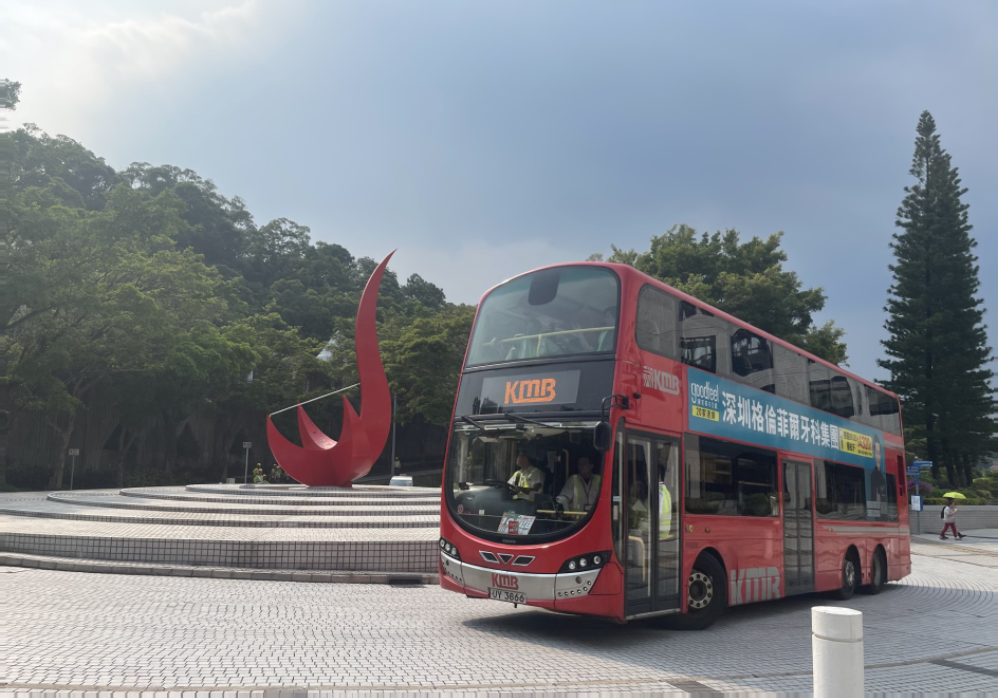
\includegraphics[width=0.8\textwidth]{images/2-method/caption-example.png}
    \caption{An example image passed through the captioning test, extracted from an email issued by HKUST to university members about transport arrangements. \\
            Caption from the CLIP-based model: `the bus is a popular tourist attraction' (score: 0.25) \\
            Enhanced caption: `The bus is an important transport option for students, offering a direct service to the campus on the 91B route.' (score: 1) }
\end{figure}

\begin{table}[!htp]
    \doublespacing
    \centering
    \caption{Accuracy statistics of different methods}
    \begin{tabular}{cccc}
        \toprule
        & CLIP-based Model & CLIP-based (Enhanced) & Multimodal LLM \\
        \midrule
        Document 1 \\(specific mathematical figures) & 0.0313 & 0.5156 & \textbf{0.9844} \\
        Document 2 \\(conceptual images) & 0.0208 & 0.4792 & \textbf{0.9792} \\
        Document 3 \\(informational images with text) & 0.1875 & 0.6875 & \textbf{0.9375} \\
        Document 4 \\(advanced concepts) & 0.25 & 0.875 & \textbf{1.0} \\
        \midrule
        Overall & 0.0588 & 0.5441 & \textbf{0.9779} \\
        \bottomrule
    \end{tabular}
\end{table}

\begin{table}[!htp]
    \doublespacing
    \centering
    \caption{Statistics on the amount of time used per image}
    \begin{tabular}{ccc}
        \toprule
        & CLIP-based Model (Enhanced) & Multimodal LLM \\
        \midrule
        Mean (s) & \textbf{2.7507} & 3.8861 \\
        Variance (s$^2$) & \textbf{1.0171} & 2.9140 \\
        Maximum (s) & \textbf{7.2277} & 10.1240 \\
        Minimum (s) & \textbf{1.7325} & 1.7750 \\
        \bottomrule
    \end{tabular}
\end{table}

\newpage
\subsubsection{Retrieval}

We use the same corpus of 4 documents from the captioning integrated tests for retrieval tests.
One of the documents from the corpus contains an introduction to a feature named ``Genmoji'', with an example ``rainbow cactus'' given.
\begin{figure}
    \centering
    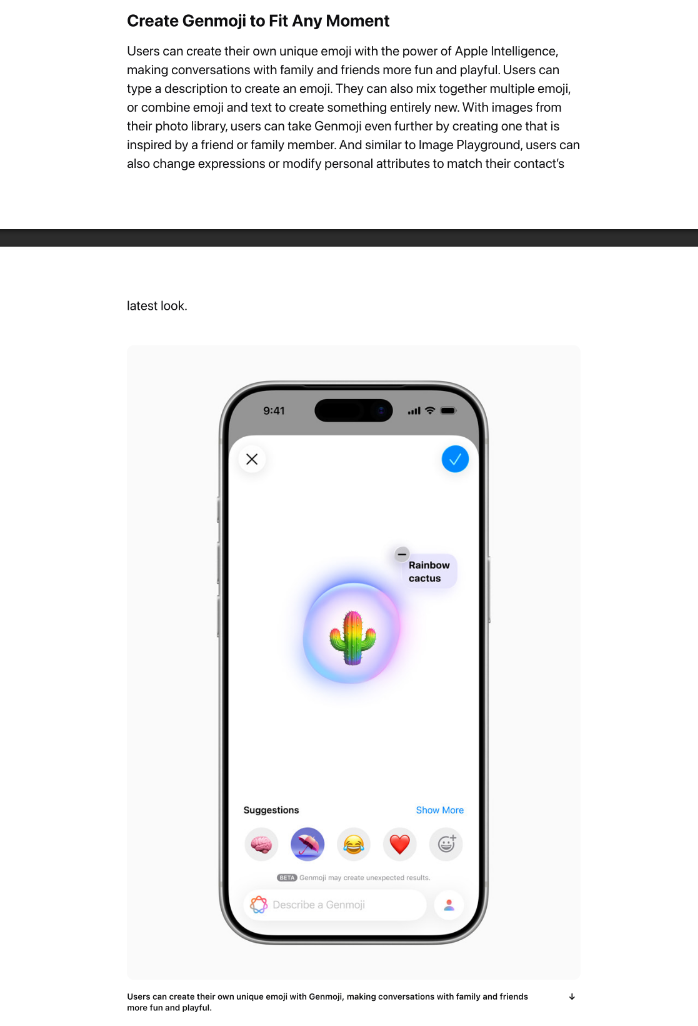
\includegraphics[width=0.8\textwidth]{images/2-method/document-example.png}
    \caption{Part of a document from the test corpus}
\end{figure}
We specifically set up a query that targets this section of the document:
\begin{verbatim}
What is Genmoji like and how can I use it? 
Can you give me an example?
\end{verbatim}

The top text chunk among the retrieval results is:
\begin{verbatim}
Retrieved document 1: 
or combine emoji and text to create something 
entirely new. With images from their photo library, 
users can take Genmoji even further by creating 
one that is inspired by a friend or family member. 
And similar to Image Playground, users can also 
change expressions or modify personal attributes to 
match their contact's latest look.
Users can create their own unique emoji with Genmoji, 
making conversations with family and friends more fun 
and playful.

Take Notes to the Next Level with Image Wand
With Image Wand in the tool palette, users can 
quickly create images in the Notes app using the 
written or visual context already captured within 
a note.
\end{verbatim}
This is correctly retrieved as the chunk mentions use cases of the ``Genmoji'' function.

With multimodal retrieval enabled, we find that the image depicting a ``rainbow cactus'' is also 
correctly retrieved and used as visual context in generating the answer.

\subsubsection{Grounding Generation Output}
\label{sec:groundingtest}

We examine the generation results of the previous example on ``Genmoji''.
One final answer when multimodal mode is enabled is
\begin{verbatim}
Genmoji is a fun feature that allows users to create 
personalized emojis for their conversations. You can 
design your own unique emoji by typing in a description 
or mixing and matching existing emojis. This feature 
adds a playful touch to your messaging, making it more 
engaging with family and friends.

For example, you can create a "rainbow cactus" emoji 
by describing it, and then you can further customize 
it by adjusting colors or combining it with other elements. 
You can also use photos from your library to inspire 
your designs, allowing for even more creative possibilities.

Overall, Genmoji is all about enhancing communication 
through visually appealing and personalized emojis 
that reflect your style and the context of your 
conversations.
\end{verbatim}
This answer correctly utilizes retrieved context to generate a comprehensive answer on the functionality of ``Genmoji'',
and provides a correct example, which was also present in the retrieved context.

We also check the results for when text-only retrieval is allowed, and for zero-shot generation.
The same text chunks are retrieved for text-only retrieval,
resulting in the following final answer:
\begin{verbatim}
Genmoji is a fun and creative feature that allows you 
to create your own unique emojis. You can make conversations 
with family and friends more playful by using Genmoji to 
craft emojis that reflect your personal style or express 
your feelings. 

To use Genmoji, you can type a description of what you 
want the emoji to look like, mix together multiple 
existing emojis, or even combine emoji and text to create 
something entirely new. Additionally, you can use images 
from your photo library to inspire your creations, 
such as designing an emoji that resembles a friend 
or family member.

For example, if you wanted to create an emoji inspired 
by your friend who loves cats, you might start by mixing 
a cat emoji with a party hat emoji to reflect their fun 
personality. You could describe it in your own words, 
like "A cat with a colorful party hat," and Genmoji 
would help you bring that idea to life!
\end{verbatim}
This answer is also correct as the retrieved text chunks contain fully the information to answer this question,
and since visual evidence does not play a very big role in the second subquestion asking for examples,
which is a more open-ended and creative question.
We can also see that the example given here does not follow the source document image example ``rainbow cactus'', 
as the model has no access to such visual context during generation.

As for zero-shot generation, the generated answer is
\begin{verbatim}
Genmoji is a creative tool that allows users to generate 
personalized emojis and stickers based on their 
preferences or input. It's often used for fun and 
self-expression, enabling users to create custom emoji 
that represent their personality or emotions in a 
more tailored way than standard emojis.

### How to Use Genmoji:

1. **Access the Platform**: Visit the Genmoji 
website or app where the service is available.
   
2. **Select Options**: You may have options to choose 
various features such as facial expressions, accessories, 
hairstyles, and backgrounds.

3. **Customize Your Emoji**: Use the provided tools to 
customize your emoji to your liking. You can usually 
adjust colors, add features, or apply different styles.

4. **Save or Share**: After creating your emoji, you 
can save it to your device or share it on social media 
platforms.

### Example:

Let's say you're feeling happy and want an emoji that 
reflects that:

1. **Choose a Base Expression**: Start with a 
    smiling face.
2. **Add Accessories**: Put on some sunglasses 
    and a party hat.
3. **Customize Colors**: Change the skin tone 
    to match yours.
4. **Finalize and Share**: Save this emoji to your 
    phone and use it in messages to friends or on 
    social media to express your cheerful mood!

By using Genmoji, you can create unique representations 
of yourself or your feelings, making communication 
more vibrant and personal.
\end{verbatim}
We find multiple issues in this answer.
For instance, the said ``Genmoji'' feature in the source document does not refer to a website application,
yet this zero-shot generated answer confidently states that access to ``Genmoji'' is via a website.

We formulate another small corpus of 4 documents for more comprehensive testing on visual retrieval and grounding.
Dataset questions are crafted using document content, targetting specific visual elements found in the document.
More details on the dataset and corpus can be found in Appendix~\ref{appendix:integrationtests} \nameref{appendix:integrationtests}.

The results by running zero-shot, text-only retrieval, and multimodal retrieval on GPT-4o-mini are as follows.
We provide tuples of scores representing (dense retrieval, graph retrieval) scores.
\begin{center}
    \begin{tabular}{ccc}
        \toprule
        Value of $k$ & Text-only & Multimodal \\
        \midrule
        0 (Zero-shot) & 27.3 & -- \\
        1 & 36.4, 9.1 & \textbf{45.5}, 18.2 \\
        3 & 36.4, 18.2 & \textbf{45.5}, \textbf{45.5} \\
        5 & \textbf{45.5}, 18.2 & 27.3, 27.3 \\
        7 & 36.4, 9.1 & \textbf{54.6}, 9.1 \\
        10 & 45.5, 18.2 & \textbf{54.6}, 36.4 \\
        15 & \textbf{45.5}, 9.1 & 27.3, 18.2 \\
        20 & \textbf{45.5}, 9.1 & 36.4, 9.1 \\
        \bottomrule
    \end{tabular}
\end{center}

We see that the level of accuracy increases from zero-shot to text-only retrieval, then to multimodal retrieval.

\subsubsection{Ablation Tests}
\label{sec:ablationtests}

\paragraph{CLIP vs DINOv2 Embeddings}
We perform ablation tests on the corpus of 4 documents used in Section~\ref{sec:groundingtest} \nameref{sec:groundingtest}
for using CLIP embeddings in multimodal embedding and retrieval.
To accomodate long-context strings, we use Long-CLIP \cite{10.1007/978-3-031-72983-6_18} instead of the vanilla CLIP model.

Test results are as follows.
Tuples of scores represent (dense retrieval, graph retrieval) scores.
\begin{center}
    \begin{tabular}{cccc}
        \toprule
        Value of $k$ & Text-only & Multimodal (DINOv2-Talk2DINO) & Multimodal (Long-CLIP) \\
        \midrule
        0 (Zero-shot) & 27.3 & -- & -- \\
        1 & 36.4, 9.1 & \textbf{45.5}, 18.2 & 36.4, 18.2 \\
        3 & 36.4, 18.2 & \textbf{45.5}, \textbf{45.5} & \textbf{45.5}, 18.2 \\
        5 & \textbf{45.5}, 18.2 & 27.3, 27.3 & \textbf{45.5}, 27.3 \\
        7 & 36.4, 9.1 & \textbf{54.6}, 9.1 & 27.3, 9.1 \\
        10 & 45.5, 18.2 & \textbf{54.6}, 36.4 & 27.3, 36.4 \\
        15 & \textbf{45.5}, 9.1 & 27.3, 18.2 & 36.4, 18.2 \\
        20 & \textbf{45.5}, 9.1 & 36.4, 9.1 & 36.4, 18.2 \\
        \bottomrule
    \end{tabular}
\end{center}
\vspace{5mm}

The DINOv2-Talk2DINO method achieves higher accuracy for $k$=1, 3, 7, 10 as compared to using CLIP (Long-CLIP) for multimodal embeddings, 
and we also note that the highest accuracy among all settings is under the DINOv2-Talk2DINO pipeline.
For larger values of $k$ such as $k$=15 and 20, text-only retrieval outperforms multimodal retrieval.
This suggests that although visual retrieval provides fine-grained visual information for smaller retrieval sets,
larger batches may introduce noise from irrelevant retrieved items, confusing the MLLM and resulting in lower accuracy.
Long-CLIP multimodal embedding retrieval underperforms DINOv2 in most settings, 
as the unified representation space for text and images loses fine-grained details for semantic alignment.

These results validate our design decision to use separate representations and dual modality retrieval, 
especially when the number of retrieved items remains moderate, such as for $k \leq 15$.

\paragraph{HyDE}
We perform experiments on comparing accuracy results between using HyDE or raw query embeddings for dense retrieval.
Our results are as follows, where scores are in tuples (using HyDE, using raw query).
\begin{center}
    \begin{tabular}{ccc}
        \toprule
        Value of $k$ & Text-only & Multimodal \\
        \midrule
        0 (Zero-shot) & 27.3 & -- \\
        1 & 36.4, 27.3 & 45.5, \textbf{54.6} \\
        3 & 36.4, \textbf{54.6} & 45.5, 36.4 \\
        5 & \textbf{45.5}, 36.4 & 27.3, \textbf{45.5} \\
        7 & 36.4, 45.5 & \textbf{54.6}, 45.5 \\
        10 & 45.5, 36.4 & \textbf{54.6}, 36.4 \\
        15 & \textbf{45.5}, 36.4 & 27.3, 36.4 \\
        20 & \textbf{45.5}, 36.4 & 36.4, 36.4 \\
        \bottomrule
    \end{tabular}
\end{center}

Among the 14 tested settings,
retrieval with HyDE won in 8, while retrieval using the raw query won in 5, and there was one tie.
No clear trend with respect to $k$ was observed.
For instance, using the raw query for retrieval gave better performance at $k$=1 in multimodal retrieval, but worse in text-only retrieval.
Given these results that lack a clear conclusion for the better method, and an additional computation cost in generating the hypothetical document under HyDE,
we leave both methods as a configurable option for flexibility.

\paragraph{Note on Dataset}
We also note that this test dataset of 4 documents and 11 queries is a small dataset, and may introduce bias in test results.
However, this small-scale testing allows us to perform deeper investigations on failed cases.

A more comprehensive evaluation using research benchmarks can be found in Section~\ref{sec:evaluation} \nameref{sec:evaluation}.


\newpage
\subsection{Evaluation}
\label{sec:evaluation}

To evaluate overall pipeline performance, we run our pipeline through benchmarks.
We examine retrieval accuracy and end-to-end answer generation on the benchmarks Visual-RAG and MMDocRAG.

\subsubsection{Benchmarks}

We present results of running our system on various benchmarks as compared to the original papers by using GPT-4o-mini\footnote{Provided by Microsoft Azure via HKUST GenAI Platform.} 
and Qwen2.5VL with our pipeline.
Accuracy scores shown below are obtained using the LLM-as-judge technique \cite{gu2025surveyllmasajudge}.
The prompt used in LLM-as-judge evaluation is listed in Appendix~\ref{appendix:prompts} \nameref{appendix:prompts}.

\paragraph{Visual-RAG}

Items in brackets represent results from the original paper.
Visual-RAG specifically targets visual elements, hence there is no text corpus; only images are indexed.
Top-$k$ retrieval refers to retrieval of the top $k$ most similar images to the query based on our metric.
Note that the original paper does not provide results for GPT-4o-mini.
We cite scores for GPT-4o from the original paper as a reference.

\begin{tabularx}{\textwidth}{@{} c | c c @{}}
    \toprule
    Model & GPT-4o-mini (GPT-4o) & Qwen2.5VL \\
    \midrule
    \endhead
    Zero-shot (no image) & 43.05 (49.33) & 56.68 (34.84) \\
    \midrule
    Top-$k$, $k$=1 & 7.49 (22.65) & 37.43 (37.96) \\
    Top-$k$, $k$=3 & 11.76 (38.50) & 33.42 (39.44) \\
    Top-$k$, $k$=5 & 15.24 (43.45) & 39.57 (39.84) \\
    Top-$k$, $k$=7 & 14.44 (46.52) & 40.91 (38.99) \\
    Top-$k$, $k$=10 & 17.11 (46.93) & 42.25 (42.91) \\
    Top-$k$, $k$=15 & 19.25 (47.33) & 46.79 (42.78) \\
    Top-$k$, $k$=20 & 17.91 (50.00) & 43.58 (43.44) \\
    \bottomrule
\end{tabularx}

Due to limits on compute resources and time, we do not use the full image dataset of 2.7M images from the iNaturalist 2021 Competition training set \cite{Van_Horn_2021_CVPR},
as in the original paper; instead we simulate the experiment with the test set of 100,000 images.
We find that Qwen2.5VL gives comparable results to the original paper although the number of ground truth images for each query is largely reduced.
We also notice that scores for GPT-4o-mini lag behind GPT-4o.

We perform further analysis on retrieval results.
We report numbers for $k$=7 and 15 additionally.
Results compared to the original paper are as follows:
\begin{tabularx}{\textwidth}{ l | r r r r r r }
    \toprule
    \textbf{Ours} & @1 & @5 & @7 & @10 & @15 & @20 \\
    \midrule
    Recall & 3.40 & 18.37 & 22.75 & 25.29 & 28.13 & 30.43 \\
    NDCG & 33.96 & 35.58 & 31.44 & 22.16 & 21.93 & 22.07 \\
    Hit & 33.96 & 70.86 & 70.86 & 70.86 & 76.47 & 76.47 \\
    Hit Count & 0.34 & 1.84 & 2.28 & 2.53 & 2.81 & 3.04 \\
    \midrule
    \textbf{CLIP} & @1 & @5 & @7 & @10 & @15 & @20 \\
    \midrule
    Recall & 2.81 & 10.26 & -- & 16.70 & -- & 25.54 \\
    NDCG & 24.33 & 25.97 & -- & 30.98 & -- & 39.21 \\
    Hit & 24.33 & 53.74 & -- & 67.65 & -- & 77.54 \\
    Hit Count & 0.24 & 1.01 & -- & 1.84 & -- & 3.18 \\
    \midrule
    \textbf{BGE} & @1 & @5 & @7 & @10 & @15 & @20 \\
    \midrule
    Recall & 3.63 & 12.43 & -- & 18.81 & -- & 28.64 \\
    NDCG & 26.74 & 29.15 & -- & 33.4 & -- & 41.83 \\
    Hit & 26.74 & 58.56 & -- & 68.98 & -- & 79.14\\
    Hit Count & 0.27 & 1.17 & -- & 2.04 & -- & 3.43 \\
    \midrule
    \textbf{VLM2Vec} & @1 & @5 & @7 & @10 & @15 & @20 \\
    \midrule
    Recall & 2.91 & 10.01 & -- & 16.03 & -- & 26.37 \\
    NDCG & 24.87 & 26.33 & -- & 30.09 & -- & 39.13 \\
    Hit & 24.87 & 51.87 & -- & 62.83 & -- & 78.34 \\
    Hit Count & 0.25 & 1.10 & -- & 1.91 & -- & 3.33 \\
    \bottomrule
\end{tabularx}

The above results are analysis results of retrieval logs from the end-to-end generation experiment.
We use the same evaluation metrics on retrieval results as the original paper, including the following:
\begin{itemize}
    \item Recall @$k$: the fraction of ground truth images among the top $k$ retrieved images
    \item Normalized Discounted Cumulative Gain (NDCG) @$k$: reflects ranking quality by rewarding correct images that appear higher in the ranking,
            by discounting relevance logarithmically with position
    \item Hit @$k$: the probability of at least one clue image among the top $k$ images
    \item Hit Count @$k$: the number of clue images found in the top $k$ retrieved images
\end{itemize}

We note that experiment conditions slightly differ from the original paper.
In retrieval evaluation, the authors of the original paper select 200 to 300 images for retrieval per question;
while we perform retrieval among all 100,000 images in the test image dataset used in our experiments,
making our experiment conditions more difficult for the retriever.

The above results show that our DINOv2-Talk2DINO pipeline provides competitive recall compared to methods tested in the paper.
However, due to a smaller ground truth set, where each species has only 10 ground truth images, and a much larger corpus, 
our NDCG values decline for $k > 5$.

Our results suggest that using DINOv2 representations and aligning textual queries with them using Talk2DINO may allow some 
minor fine-grained visual details to be considered in the retrieval process.

\newpage
\paragraph{MMDocRAG}

Items in brackets represent output factuality score results from the original paper.
We provide scores for zero-shot and $k$=5, 7 and 10 additionally.

\begin{tabularx}{\textwidth}{@{} c | c c @{}}
    \toprule
    Model & GPT-4o-mini & Qwen2.5VL\footnote{For pure-text evaluations, the original paper provides results from \verb|Qwen2.5-7B-Inst|. We compare with such results.} \\
    \midrule
    \endhead
    \multicolumn{3}{c}{Pure-text input sequence to MLLM} \\
    \midrule
    Zero-shot (no retrieval) & 49.9 (--) & 69.2 (--) \\
    \midrule
    5 quotes\footnote{`Quotes' refers to the number of retrieved passages. \label{mmdocragquotes}} (Top-$k$, $k$=5) & 50.4 (--) & 59.6 (--) \\
    7 quotes\textsuperscript{\ref{mmdocragquotes}} (Top-$k$, $k$=7) & 51.1 (--) & 59.8 (--) \\
    10 quotes\textsuperscript{\ref{mmdocragquotes}} (Top-$k$, $k$=10) & 54.0 (--) & 61.0 (--) \\
    15 quotes\textsuperscript{\ref{mmdocragquotes}} (Top-$k$, $k$=15) & 56.9 (70.0) & 61.8 (61.2) \\
    20 quotes\textsuperscript{\ref{mmdocragquotes}} (Top-$k$, $k$=20) & 57.4 (69.8) & 62.0 (61.4) \\
    \midrule
    \multicolumn{3}{c}{Multimodal input sequence to MLLM} \\
    \midrule
    5 quotes\textsuperscript{\ref{mmdocragquotes}} (Top-$k$, $k$=5) & 52.7 (--) & 65.8 (--) \\
    7 quotes\textsuperscript{\ref{mmdocragquotes}} (Top-$k$, $k$=7) & 55.6 (--) & 66.4 (--) \\
    10 quotes\textsuperscript{\ref{mmdocragquotes}} (Top-$k$, $k$=10) & 55.6 (--) & 67.0 (--) \\
    15 quotes\textsuperscript{\ref{mmdocragquotes}} (Top-$k$, $k$=15) & 57.5 (66.7) & 66.4 (63.2) \\
    20 quotes\textsuperscript{\ref{mmdocragquotes}} (Top-$k$, $k$=20) & 55.5 (64.6) & 65.8 (62.6) \\
    \bottomrule
\end{tabularx}

We note that our results on GPT-4o-mini lag behind the original paper; yet results on Qwen2.5VL outperforms the original paper in most settings.
This phenomenon may be due to performance differences between GPT-4o-mini offered by Microsoft Azure\footnote{We use GPT-4o-mini offered by Microsoft Azure through HKUST GenAI Platform.}
and the official GPT-4o-mini from OpenAI, or model versioning differences.
Although generation with retrieval only provides marginal gains over zero-shot generation for GPT-4o-mini,
the factuality scores increase as more items are retrieved and used as context.
This trend indicates that more provided context aids generation in a correct direction.

The results for Qwen2.5VL further validate that our DINOv2-Talk2DINO pipeline provides the MLLM with useful multimodal context extracted from document images,
such as graphs, tables, and explanatory images.

\paragraph{Discussion on Zero-Shot Generation}
We find that zero-shot generation for both Visual-RAG and MMDocRAG with Qwen gives higher accuracy than outputs under retrieval;
whereas scores for GPT-4o-mini follow the expected trend and increase as more items are being retrieved.
We hypothesize that post-training with Supervised Fine-Tuning (SFT) on Qwen2.5 to achieve long-context generation 
and logical reasoning abilities \cite{qwen2025qwen25technicalreport} causes this phenomenon.
Longer zero-shot generation output has a higher chance of hitting related factual points presented in the ground truth answers,
leading to the LLM judge awarding more points to zero-shot answers.
Generation with retrieval does not benefit from these model characteristics as we prompt for generation to be strictly based on retrieved context.

\subsubsection{Overall Evaluation}

Our evaluation of the overall pipeline with the following criteria is as follows:
\begin{enumerate}
    \item Is the collected dataset large enough to evaluate the pipeline thoroughly? \\
            We mainly use MMDocRAG and Visual-RAG as evaluation benchmarks. 
            MMDocRAG contains 222 long documents and 4,055 expert-annotated question-answer pairs, 
            while Visual-RAG utilizes a dataset of 2.7M images and 374 queries that require retrieval based on fine-grained visual details.
            This is sufficient to evaluate our pipeline's performance.

    \item Does the designed embedding strategy retain sufficient necessary information from the raw multimodal data? \\
            We find that retrieval accuracy is high enough to ground generation in a correct direction, 
            with multimodal data and textual data both used.
            This can be seen in our tests, where for a moderate number of multimodal retrieved items (such as $k$=7, 10),
            multimodal retrieval gives better accuracy than text-only retrieval.
            Benchmarking results with MMDocRAG also reveal the same.
            This suggests that the encoding method provides meaningful embeddings that can be retrieved correctly for use.

    \item Is the storage mechanism efficient enough to provide quick retrieval upon actual use with a MLLM? \\
            We observe that the vector database storage option allows retrieval of documents very rapidly in seconds, 
            which is ideal performance for retrieval and passing to a MLLM for generation.
            The knowledge graph-based storage option takes slightly longer to retrieve items due to embedding community summaries on the spot;
            yet theoretically this option preserves long-form context better.
            Our test results, however, do not support this.
            The choice of storage mechanism lies within the actual use case of this system,
            and we leave the choice as a configurable option in our pipeline.

    \item How relevant is the retrieved information when compared to the input query? \\
            As observed in our tests and experiments, we find that retrieval using the HyDE technique or the raw query both allow
            effective retrieval of relevant text chunks and images.
            Our prompts also instruct the MLLM to strictly generate answers only based on retrieved items.
            Answer accuracy is an indicator for retrieval effectiveness in our tests.
            We note that retrieval increases accuracy compared to zero-shot baselines in all tests and benchmarks,
            hence we conclude that retrieved items can successfully ground generation and can largely reduce hallucination.

    \item How helpful is the system in reducing hallucinations or factual errors when dealing with multimodal data? \\
            Following from the previous question, relevant text chunks and images can successfully and correctly be retrieved prior to generation.
            The prompt for the final answer instructs the MLLM to appropriately utilize the provided retrieved context in answering the input query,
            and we find that grounded generation provides ideal performance in preventing hallucinations or factual errors. 
            However, we also find that when too many retrieved multimodal items are retrieved and used as context,
            the MLLM may get confused and consequently produce incorrect answers.
            The optimal values of $k$ from our empirical results are $k$=7, 10 or 15.

    \newpage
    \item How does this system compare to emerging research papers on similar topics? \\
            Our benchmark results on MMDocRAG are on par with results from the original paper,
            and exceed original results in certain settings.
            We also find that our results on Qwen2.5VL are comparable to the original paper results in Visual-RAG,
            and further analysis on retrieval results shows that our method gives slightly better retrieval performance.
\end{enumerate}